\section{FreeCell prank (Windows 7)}

\renewcommand{\CURPATH}{examples/freecell}

This is a prank I once played for my coworkers who played FreeCell solitaire too much.
Can we make FreeCell always deal the same game each time?
Like, you know, in ``Groundhog Day'' movie?

(I'm writing this in November 2019. Somehow, IDA can't get PDBs from Microsoft servers. Maybe Windows 7 is unsupported anymore?
Anyway, I can't get function names...)

\subsection{Part I}

\myindex{\CStandardLibrary!rand()}
\myindex{\CStandardLibrary!srand()}
\myindex{\CStandardLibrary!time()}
So I loaded FreeCell.exe into IDA and found that both rand(), srand() and time() are imported from msvcrt.dll.
time() is indeed used as a seed for srand():

\begin{lstlisting}[style=customasmx86]
.text:01029612                sub_1029612     proc near               ; CODE XREF: sub\_102615C+149
.text:01029612                                                        ; sub\_1029DA6+67
.text:01029612 8B FF                          mov     edi, edi
.text:01029614 56                             push    esi
.text:01029615 57                             push    edi
.text:01029616 6A 00                          push    0               ; Time
.text:01029618 8B F9                          mov     edi, ecx
.text:0102961A FF 15 80 16 00+                call    ds:time
.text:01029620 50                             push    eax             ; Seed
.text:01029621 FF 15 84 16 00+                call    ds:srand
.text:01029627 8B 35 AC 16 00+                mov     esi, ds:rand
.text:0102962D 59                             pop     ecx
.text:0102962E 59                             pop     ecx
.text:0102962F FF D6                          call    esi ; rand
.text:01029631 FF D6                          call    esi ; rand
.text:01029633
.text:01029633                loc_1029633:                            ; CODE XREF: sub\_1029612+26
.text:01029633                                                        ; sub\_1029612+2D
.text:01029633 FF D6                          call    esi ; rand
.text:01029635 83 F8 01                       cmp     eax, 1
.text:01029638 7C F9                          jl      short loc_1029633
.text:0102963A 3D 40 42 0F 00                 cmp     eax, 1000000
.text:0102963F 7F F2                          jg      short loc_1029633
.text:01029641 6A 01                          push    1
.text:01029643 50                             push    eax
.text:01029644 8B CF                          mov     ecx, edi
.text:01029646 E8 2D F8 FF FF                 call    sub_1028E78
.text:0102964B 5F                             pop     edi
.text:0102964C 5E                             pop     esi
.text:0102964D C3                             retn
.text:0102964D                sub_1029612     endp
\end{lstlisting}

Several (redundant) calls to rand() are funny, that reminds me:

``In the morning you will send for a hansom, desiring your man to take neither the first nor the second which may present itself.''
( The Memoirs of Sherlock Holmes, by Arthur Conan Doyle\footnote{\url{http://www.gutenberg.org/files/834/834-0.txt}} )

There is another call of time() and srand() pair, but my \tracer showed that this is the point of our interest:

\begin{lstlisting}
tracer.exe -l:FreeCell.exe bpf=msvcrt.dll!time bpf=msvcrt.dll!srand,args:1

...

TID=5340|(0) msvcrt.dll!time() (called from FreeCell.exe!BASE+0x29620 (0x209620))
TID=5340|(0) msvcrt.dll!time() -> 0x5ddb68aa
TID=5340|(1) msvcrt.dll!srand(0x5ddb68aa) (called from FreeCell.exe!BASE+0x29627 (0x209627))
TID=5340|(1) msvcrt.dll!srand() -> 0x5507e0
TID=5340|(1) msvcrt.dll!srand(0x399f) (called from FreeCell.exe!BASE+0x27d3a (0x207d3a))
TID=5340|(1) msvcrt.dll!srand() -> 0x5507e0
\end{lstlisting}

You see, the time() function returned 0x5ddb68aa and the very same value is used as an argument for srand().

Let's try to force time() to always return 0:

\begin{lstlisting}
tracer.exe -l:FreeCell.exe bpf=msvcrt.dll!time,rt:0 bpf=msvcrt.dll!srand,args:1

...

TID=2104|(0) msvcrt.dll!time() (called from FreeCell.exe!BASE+0x29620 (0xb19620))
TID=2104|(0) msvcrt.dll!time() -> 0x5ddb68f6
TID=2104|(0) Modifying EAX register to 0x0
TID=2104|(1) msvcrt.dll!srand(0x0) (called from FreeCell.exe!BASE+0x29627 (0xb19627))
TID=2104|(1) msvcrt.dll!srand() -> 0x3707e0
TID=2104|(1) msvcrt.dll!srand(0x52f6) (called from FreeCell.exe!BASE+0x27d3a (0xb17d3a))
TID=2104|(1) msvcrt.dll!srand() -> 0x3707e0
\end{lstlisting}

Now I'm seeing the same game each time I'm running FreeCell using \tracer:

\begin{figure}[H]
\centering
\frame{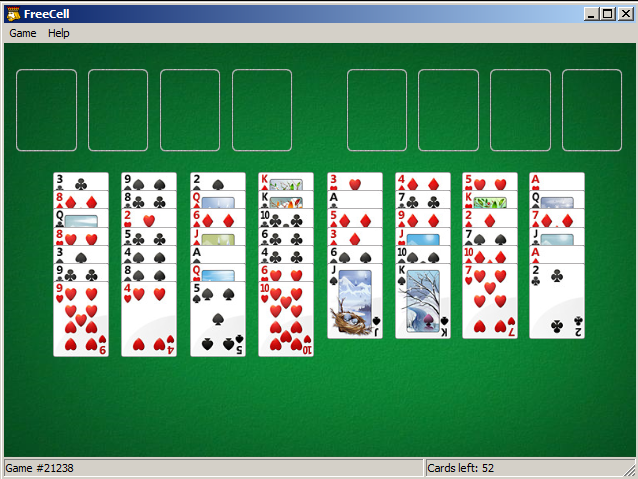
\includegraphics[width=1.0\textwidth]{\CURPATH/freecell1.png}}
\end{figure}

Now how to patch the executable?

We want to pass 0 as an argument to srand() at 0x01029620.
But there is a one-byte instruction: \INS{PUSH EAX}.
\INS{PUSH 0} is two-byte instruction. How to squeeze it into?

What is in other registers at this moment? Using \tracer I'm dumping all them:

\begin{lstlisting}
tracer.exe -l:FreeCell.exe bpx=FreeCell.exe!0x01029620

...

TID=4448|(0) FreeCell.exe!0x1029620
EAX=0x5ddb6ac4 EBX=0x00000000 ECX=0x00000000 EDX=0x00000000
ESI=0x054732d0 EDI=0x054732d0 EBP=0x0020f2bc ESP=0x0020f298
EIP=0x00899620
FLAGS=PF ZF IF
TID=4448|(0) FreeCell.exe!0x1029620
EAX=0x5ddb6ac8 EBX=0x00000002 ECX=0x00000000 EDX=0x00000000
ESI=0xffffff11 EDI=0x054732d0 EBP=0x0020da78 ESP=0x0020d9d4
EIP=0x00899620
FLAGS=PF ZF IF
TID=4448|(0) FreeCell.exe!0x1029620
EAX=0x5ddb6aca EBX=0x00000002 ECX=0x00000000 EDX=0x00000000
ESI=0x7740c460 EDI=0x054732d0 EBP=0x0020da78 ESP=0x0020d9d4
EIP=0x00899620
FLAGS=PF ZF IF
...
\end{lstlisting}

No matter how often I restart the game, ECX and EDX are seems to be always 0.
So I patching \INS{PUSH EAX} at 0x01029620 to \INS{PUSH EDX} (also one-byte instruction),
and now FreeCell always shows the same game to the player.

However, other options could exist.
As a matter of fact, we don't need to pass 0 to srand().
Rather, we want to pass a \emph{constant} to srand() to make game the same each time.
As we can see, EDI's value hasn't been changing. Maybe we could try it as well.

Now a bit harder patching.
Let's open FreeCell.exe in Hiew:

\begin{figure}[H]
\centering
\frame{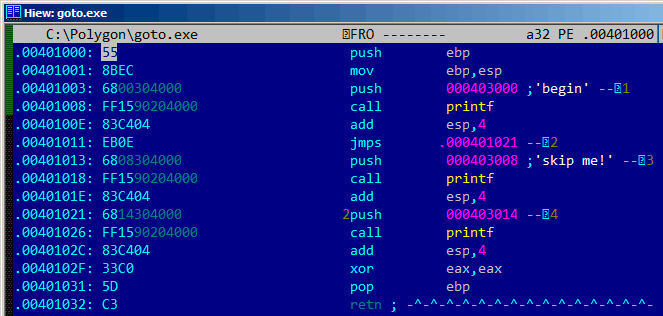
\includegraphics[width=1.0\textwidth]{\CURPATH/hiew1.png}}
\end{figure}

We have no space to replace one-byte \INS{PUSH EAX} with two-byte \INS{PUSH 0}.
\myindex{FIXUP}
And we can't simply fill \verb|CALL ds:time| with \ac{NOP}s, because there is a FIXUP (address of time() function in msvcrt.dll).
(Hiew marked these 4 bytes are gray bytes.)
So what I'm doing: patching first 2 bytes to EB 04. This is a \INS{JMP} to bypass 4 FIXUP-ed bytes:

\begin{figure}[H]
\centering
\frame{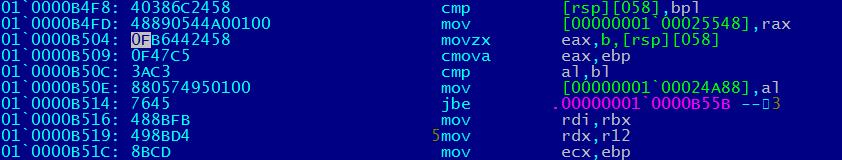
\includegraphics[width=1.0\textwidth]{\CURPATH/hiew2.png}}
\end{figure}

Then I replace \INS{PUSH EAX} with \ac{NOP}. So that srand() would have its zeroes arguments from \INS{PUSH 0} above.
Also, I patch one of \INS{POP ECX} to \ac{NOP}, because I removed one \INS{PUSH}.

\begin{figure}[H]
\centering
\frame{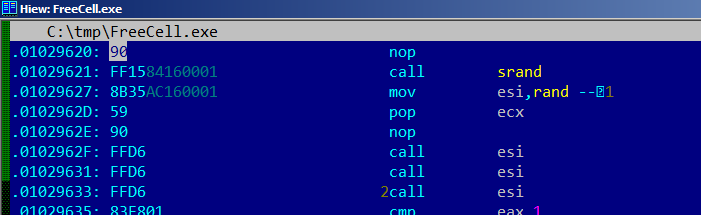
\includegraphics[width=1.0\textwidth]{\CURPATH/hiew3.png}}
\end{figure}

Now Windows loader will write 4-byte FIXUP at 0x0102961C, but we don't care: time()'s address will not be used anymore.

\subsection{Part II: breaking the \emph{Select Game} submenu}

The user can still choose different game in the menu.
Let's see if srand() is still called.
I'm trying to enter 1/2/3 in "Select Game" dialog box:

\begin{lstlisting}
tracer.exe -l:FreeCell.exe bpf=msvcrt.dll!srand,args:1

...

TID=4936|(0) msvcrt.dll!srand(0x5ddb6df9) (called from FreeCell.exe!BASE+0x29627 (0xb49627))
TID=4936|(0) msvcrt.dll!srand() -> 0x5907e0
TID=4936|(0) msvcrt.dll!srand(0x2b40) (called from FreeCell.exe!BASE+0x27d3a (0xb47d3a))
TID=4936|(0) msvcrt.dll!srand() -> 0x5907e0
TID=4936|(0) msvcrt.dll!srand(0x1) (called from FreeCell.exe!BASE+0x27d3a (0xb47d3a))
TID=4936|(0) msvcrt.dll!srand() -> 0x5907e0
TID=4936|(0) msvcrt.dll!srand(0x2) (called from FreeCell.exe!BASE+0x27d3a (0xb47d3a))
TID=4936|(0) msvcrt.dll!srand() -> 0x5907e0
TID=4936|(0) msvcrt.dll!srand(0x3) (called from FreeCell.exe!BASE+0x27d3a (0xb47d3a))
TID=4936|(0) msvcrt.dll!srand() -> 0x5907e0
\end{lstlisting}

Yes, the number user enters is just an argument for srand().
Where it is called?

\begin{lstlisting}
.text:01027CBA                loc_1027CBA:                            ; CODE XREF: sub\_1027AC6+179
.text:01027CBA 83 FF FC                       cmp     edi, 0FFFFFFFCh
.text:01027CBD 75 74                          jnz     short loc_1027D33

...

.text:01027D33                loc_1027D33:                            ; CODE XREF: sub\_1027AC6+1F7
.text:01027D33 57                             push    edi             ; Seed
.text:01027D34 FF 15 84 16 00+                call    ds:srand
.text:01027D3A 59                             pop     ecx
.text:01027D3B 6A 34                          push    34h
.text:01027D3D 5B                             pop     ebx
.text:01027D3E 33 C0                          xor     eax, eax
\end{lstlisting}

I couldn't patch one-byte \INS{PUSH EDI} to two-byte \INS{PUSH 0}.
But I see that there is only one single jump to \verb|loc_1027D33| from the above.

I'm patching \INS{CMP EDI, ...} to \INS{XOR EDI, EDI}, padding the 3rd byte to \ac{NOP}.
I'm patching also JNZ to JMP, so that jump will always occur.

Now FreeCell ignores the number user enters, but suddenly, there is also the same game at start:

\begin{figure}[H]
\centering
\frame{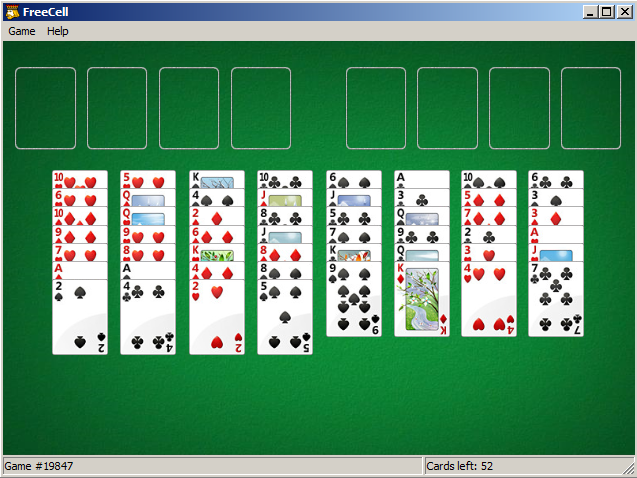
\includegraphics[width=1.0\textwidth]{\CURPATH/freecell2.png}}
\end{figure}

It seems that the code we patched in part I is somehow connected to a code after 0x01027CBD, that executes if EDI==0xFFFFFFFC.
Anyway, our goal is accomplished --- the game is always the same at the start and the user can't choose another using the menu.
